\documentclass[12pt,a4paper]{article}
\usepackage[utf8]{inputenc}
\usepackage{amsmath}
\usepackage{geometry}
\usepackage{xcolor}
\usepackage{tcolorbox}
\usepackage{tikz}
\usepackage{multicol}
\usetikzlibrary{shapes,arrows,positioning}

\geometry{margin=0.5in}
\pagestyle{empty}

\definecolor{primaryblue}{RGB}{0,51,102}
\definecolor{accentgold}{RGB}{218,165,32}
\definecolor{treasurygreen}{RGB}{34,139,34}

\begin{document}

\begin{center}
{\Huge\textbf{\textcolor{primaryblue}{BlocTime Protocol}}}\\
\vspace{0.2cm}
{\Large\textcolor{accentgold}{Earn Passive Income from Real Marketplace Revenue}}\\
\vspace{0.1cm}
{\textit{One-Page Overview}}
\end{center}

\vspace{0.3cm}

\begin{multicols}{2}

\section*{\textcolor{primaryblue}{What is BlocTime?}}

BlocTime is a revolutionary protocol that lets you \textbf{earn passive income from a thriving marketplace} by simply locking up your tokens. Think of it as a savings account that pays dividends from real business activity, not from printing new money.

\section*{\textcolor{primaryblue}{The Simple Idea}}

\subsection*{For Token Holders}
\begin{enumerate}
    \item Lock your tokens for a period
    \item Receive BlocTime tokens (up to 3x multiplier)
    \item Earn automatic rewards from ALL marketplace fees
    \item Claim anytime without unstaking
    \item Get tokens back after lock period
\end{enumerate}

\subsection*{For Marketplace Users}
\begin{enumerate}
    \item Rent computing power, AI models, or digital assets by the block
    \item Pay only for what you use
    \item Resell unused time on secondary market
    \item Access premium resources without huge upfront costs
\end{enumerate}

\section*{\textcolor{primaryblue}{Automatic Revenue Sharing}}

Every marketplace transaction:
\begin{itemize}
    \item \textbf{97.5\%} → Resource owner
    \item \textbf{2.5\%} → Treasury → ALL stakers
\end{itemize}

\textbf{This means:}
\begin{itemize}
    \item ✅ No token inflation
    \item ✅ No manual work
    \item ✅ Fair distribution
    \item ✅ Sustainable growth
\end{itemize}

\section*{\textcolor{primaryblue}{Lock-Time Multiplier}}

\begin{center}
\begin{tabular}{|l|c|c|}
\hline
\textbf{Duration} & \textbf{Mult.} & \textbf{Example} \\
\hline
0 blocks & 1.0x & 100 → 100 \\
10k blocks & 1.5x & 100 → 150 \\
50k blocks & 2.0x & 100 → 200 \\
100k blocks & 3.0x & 100 → 300 \\
\hline
\end{tabular}
\end{center}

\textbf{More BlocTime = Bigger share of revenue}

\columnbreak

\section*{\textcolor{primaryblue}{Real Example}}

\textbf{You stake:} 1,000 tokens for 50k blocks\\
\textbf{You receive:} 2,000 BlocTime (2x multiplier)\\
\textbf{Total BlocTime:} 100,000\\
\textbf{Your share:} 2\%

\vspace{0.2cm}

If marketplace generates \textbf{\$10,000/month}:\\
→ Distribution pool: \$5,000\\
→ \textbf{Your reward: \$100/month}

\vspace{0.2cm}

\textbf{Every month, as long as marketplace is active!}

\section*{\textcolor{primaryblue}{The Virtuous Cycle}}

\begin{center}
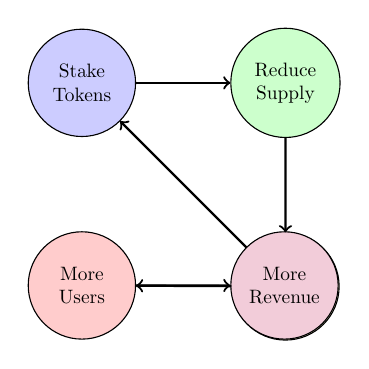
\begin{tikzpicture}[node distance=1.2cm, auto, scale=0.8, every node/.style={scale=0.7}]
  \node[draw, circle, fill=blue!20, text width=1.5cm, align=center] (stake) {Stake Tokens};
  \node[draw, circle, fill=green!20, text width=1.5cm, align=center, right=of stake] (supply) {Reduce Supply};
  \node[draw, circle, fill=yellow!20, text width=1.5cm, align=center, below=of supply] (value) {Higher Value};
  \node[draw, circle, fill=red!20, text width=1.5cm, align=center, below=of stake] (users) {More Users};
  \node[draw, circle, fill=purple!20, text width=1.5cm, align=center, right=of users] (revenue) {More Revenue};
  
  \draw[->, thick] (stake) -- (supply);
  \draw[->, thick] (supply) -- (value);
  \draw[->, thick] (value) -- (users);
  \draw[->, thick] (users) -- (revenue);
  \draw[->, thick] (revenue) -- (stake);
\end{tikzpicture}
\end{center}

\section*{\textcolor{primaryblue}{Why Different?}}

\begin{center}
\begin{tabular}{|l|c|c|}
\hline
 & \textbf{Traditional} & \textbf{BlocTime} \\
\hline
Rewards & Inflation & Revenue \\
APY & Fixed & Growth \\
Value & Dilutes & Grows \\
Work & Manual & Auto \\
\hline
\end{tabular}
\end{center}

\section*{\textcolor{primaryblue}{Security}}

✅ OpenZeppelin contracts\\
✅ ReentrancyGuard protection\\
✅ Battle-tested security\\
✅ No admin keys for core functions\\
✅ Deployed on Base network

\section*{\textcolor{primaryblue}{Get Started}}

\textbf{As Staker:}\\
1. Get tokens → 2. Stake → 3. Earn rewards

\textbf{As User:}\\
1. Browse → 2. Rent → 3. Use → 4. Resell

\end{multicols}

\vspace{0.3cm}

\begin{center}
\begin{tcolorbox}[colback=primaryblue!5,colframe=primaryblue,width=\textwidth]
\begin{center}
\textbf{\Large The BlocTime Promise}\\
\vspace{0.2cm}
\textbf{Sustainable} · \textbf{Automatic} · \textbf{Fair} · \textbf{Aligned} · \textbf{Simple}\\
\vspace{0.2cm}
{\textcolor{accentgold}{\textit{"Where Mathematics Meets Economics"}}}\\
\vspace{0.1cm}
{\textcolor{treasurygreen}{\textit{Built with 💎 by the BlocTime Team}}}
\end{center}
\end{tcolorbox}
\end{center}

\end{document}